Neural Machine Translation (NMT) achieved state-of-the-art performances in
large-scale translation tasks such as from English to French \cite{luong15} and
English to German \cite{jean15}. NMT is appealing since it requires minimal
domain knowledge and is conceptually simple. The model by \newcite{luong15} reads through all the source words until the end-of-sentence symbol \eos{} is reached. It then starts emitting one target word at a time, as illustrated in Figure~\ref{f:lstm}. NMT is often a large neural network that is trained in an end-to-end fashion and has the ability to generalize well to very long word sequences. This means the model does not have to explicitly store gigantic phrase tables and language models as in the case of standard MT; hence, NMT has a small memory footprint. Lastly, implementing NMT decoders is easy unlike the highly intricate decoders in standard MT \cite{Koehn:2003:SMT}.

\begin{figure}
\centering
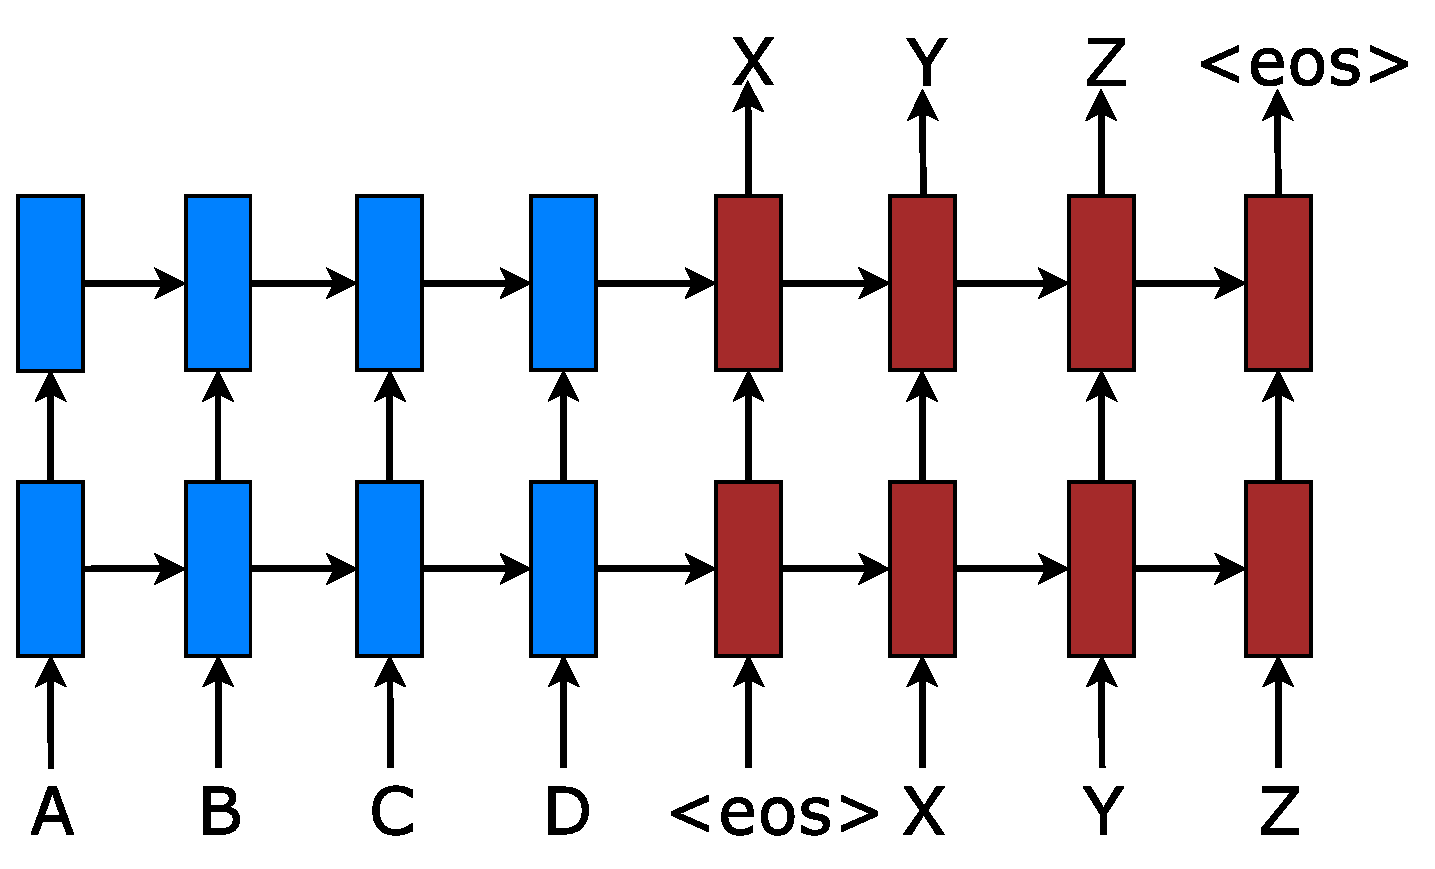
\includegraphics[width=0.45\textwidth, clip=true, trim= 0 0 0 0]{img/4-lstm} % , angle=-90
\caption[Neural machine translation]{{\bf Neural machine translation} -- a stacking recurrent architecture for translating a source sequence \texttt{A B C D} into a target sequence \texttt{X Y Z}. Here, \eos{} marks the end of a sentence.
} 
\label{f:lstm}
\end{figure}

In parallel, the concept of ``attention" has gained popularity recently in
training neural networks, allowing models to learn alignments between different
modalities, e.g., between image objects and agent actions in the dynamic control
problem \cite{mnih14}, between speech frames and text in the speech recognition
task \cite{jan14},  or between visual features of a picture and its text
description in the image caption generation task \cite{xu15}. In the context of
NMT, \newcite{bog15} has successfully applied such attentional mechanism to
jointly translate and align words. To the best of our knowledge, there has not
been any other work exploring the use of attention-based architectures for NMT.

In this work, we design, with simplicity and effectiveness in mind, two novel
types of attention-based models: a {\it global} approach in which all source
words are attended and a {\it local} one whereby only a subset of source words
are considered at a time. The former approach resembles the model of
\cite{bog15} but is simpler architecturally. The latter can be viewed as an
interesting blend between the {\it hard} and {\it soft} attention models
proposed in \cite{xu15}: it is computationally less expensive than the
global model or the soft attention; at the same time, unlike the hard attention,
the local attention is
differentiable almost everywhere, making it easier to implement and
train.\footnote{There is a recent work by \newcite{draw15}, which is very
similar to our local attention and applied to the image generation task.
However, as we detail later, our model is much simpler and can achieve good performance for NMT.} Besides, we also examine various
alignment functions for our attention-based models.

Experimentally, we demonstrate that both of our approaches are
effective in the WMT translation tasks between English and German in  both
directions. Our attentional models yield a boost of up to \attngain{} BLEU over
non-attentional systems which already incorporate known techniques such as
dropout. For English to German translation, we achieve new state-of-the-art
(SOTA)
results for both WMT'14 and WMT'15, outperforming previous SOTA systems, backed by
NMT models and $n$-gram LM rerankers, by more than 1.0 BLEU. We conduct
extensive analysis to evaluate our models in terms of learning, the ability to
handle long sentences, choices of attentional architectures, alignment quality, and translation
outputs. 
%We are also first to assess our attentional
%models using alignment error rates. 
%Moreover, we can provide the models with the information about past alignment decisions by feeding the attentional vector as an additional input to the next time step. With this minor modification, we achieve a further gain of up to \impfeed{} BLEU on top of an attention-based model.
